\documentclass[a4paper,10pt]{article}
\pdfoutput=1
%\usepackage{jheppub}
\usepackage{graphicx}% Include figure files
\usepackage{graphics}
\usepackage{dcolumn}% Align table columns on decimal point
\usepackage{bm}% bold math
\usepackage{epstopdf}
\usepackage{mathrsfs}
\usepackage{amssymb}
\usepackage{amsmath}
%\usepackage[pdftex]{hyperref}
%\usepackage{natbib}
\usepackage{multirow,cite}

\bibliographystyle{JHEP}

\def\bs{\boldsymbol}
\def\del{\partial}

%\def\p{{\boldsymbol p}_{\perp }}
%\def\pb{\bar {\boldsymbol p}_{\perp }}
%\def\pp{{\boldsymbol p}_{\perp }}
\def\p{{\boldsymbol p}}
\def\pb{\bar {\boldsymbol p}}
\def\pp{{\boldsymbol p}}
%\def\q{{\boldsymbol q}_\perp}
\def\q{{\boldsymbol q}}
\def\l{{\boldsymbol l}_\perp}
%\def\k{{\boldsymbol k}_\perp}
\def\k{{\boldsymbol k}}
\def\m{{\boldsymbol m}_\perp}
%\def\x{{\boldsymbol x}_\perp}
\def\x{{\boldsymbol x}}
\def\y{{\boldsymbol y}_\perp}
\def\X{{\boldsymbol X}_\perp}
\def\Y{{\boldsymbol Y}_\perp}
\def\D{{\boldsymbol D}_\perp}
\def\r{{\boldsymbol r}_\perp}
\def\z{{\boldsymbol z}_\perp}
%\def\v{{\boldsymbol v}_\perp}
\def\v{{\boldsymbol v}}
\def\w{{\boldsymbol w}_\perp}
\def\b{{\boldsymbol b}_\perp}
\def\Q{{\boldsymbol Q}_\perp}
\def\M{{\boldsymbol M}_\perp}
%\def\bkappa{{\boldsymbol \kappa}_\perp}
%\def\bbkappa{\bar{\boldsymbol \kappa}_\perp}
\def\bkappa{{\boldsymbol \kappa}}
\def\bbkappa{\bar{\boldsymbol \kappa}}
\def\bnu{{\boldsymbol \nu}_\perp}
\def\V{\hat{\boldsymbol v}_{1\perp}}
\def\K{\hat{\boldsymbol k}_{1\perp}}
\def\bV{\hat{\boldsymbol v}_{2\perp}}
\def\bK{\hat{\boldsymbol k}_{2\perp}}
\def\qqb{{q\bar q}}
\def\sM{{\scriptscriptstyle M}}

\newcommand{\beq}{\begin{eqnarray}}
\newcommand{\eeq}{\end{eqnarray}}
\newcommand{\be}{\begin{equation}}
\newcommand{\ee}{\end{equation}}
\newcommand{\nn}{\nonumber\\ }
\newcommand{\labe}{\label}
\newcommand{\bea}{\begin{eqnarray}}
\newcommand{\eea}{\end{eqnarray}}


\newcommand{\la}{\left\langle}
\newcommand{\ra}{\right\rangle}
\newcommand{\lc}{\left[}
\newcommand{\rc}{\right]}
\newcommand{\lp}{\left(}
\newcommand{\rp}{\right)}

%\bibliographystyle{JHEP}

%\textwidth=15.0cm \textheight=23.5cm
\textwidth=16.0cm \textheight=23.0cm 
\topmargin 0cm \oddsidemargin 0cm 
\setlength{\unitlength}{1mm}

\usepackage{url}
\usepackage{hyperref}

\begin{document}

\begin{center}
  {\Large \bf Extracting the Higgs self-coupling at a 100 TeV\\[0.2cm] hadron
  collider in the $b\bar{b}b\bar{b}$ final state}
\vspace{.7cm}

J. Katharina Behr, Daniela Bortoletto, James A. Frost,\\
  Nathan P. Hartland, Cigdem Issever and Juan Rojo


\vspace{.3cm}
{\it Physics Department, 1 Keble Road, University of Oxford, United Kingdom }

\end{center}
\vspace{0.2cm}


\paragraph{Introduction}

In this contribution we provide an estimate of the accuracy
in the Higgs self-coupling extraction that can be achieved at a 100 TeV
hadron collider in the  $b\bar{b}b\bar{b}$ final state.
%
The analysis methodology is based on our feasibility
study at 14 TeV~\cite{Behr:2015oqq}, with suitable modifications for the 100 TeV
case.
%
This strategy is based upon a combination of traditional cut-based
 methods and Multivariate Analysis (MVA).
  %
  We account for  all relevant
  backgrounds, including the contribution from mis-identified
  light and charm jets.
  %
  Our analysis strategy is found to be robust even in a high pile-up
  environment.
  %
 Our results at 14 TeV~\cite{Behr:2015oqq} indicate that 
  the $b\bar{b}b\bar{b}$ 
final state
alone should allow for the observation of double Higgs production
  at the HL-LHC, and here we study how our findings apply to the case of a 100
  TeV collider.
  %
  Other studies of Higgs pair production in the same
final state can be found in Refs.~\cite{Wardrope:2014kya,deLima:2014dta}.

\paragraph{Monte Carlo samples generation}

Higgs pair production in the gluon-fusion
channel is simulated at leading order (LO) using
{\tt MadGraph5\_aMC@NLO}~\cite{Alwall:2014hca,Maltoni:2014eza}
using a tailored  model
which includes mass effects
from the
exact form factors.
%
The calculation is performed in the
$n_f$=4 scheme and
the renormalization and factorization
scales are taken to be $\mu_F=\mu_R=H_T/2$.
%
For the input PDFs we 
adopt the NNPDF 3.0 $n_f=4$ LO set~\cite{Ball:2014uwa} with
$\alpha_s(m_Z^2)=0.118$,
interfaced via {\tt LHAPDF6}~\cite{Buckley:2014ana}.
%
To achieve the correct higher-order value of the
integrated cross-section, we rescale our LO signal sample to match the
NNLO+NNLL
inclusive calculation~\cite{deFlorian:2013jea,deFlorian:2015moa}.
%
Parton level signal events are then showered with the {\tt Pythia8} Monte
Carlo~\cite{Sjostrand:2007gs,Sjostrand:2014zea}, version {\tt v8.201},
using the  Monash 2013 tune~\cite{Skands:2014pea},
based on the NNPDF2.3LO PDF set~\cite{Ball:2012cx,Ball:2013hta}.
%
Background samples are generated at LO
with {\tt SHERPA}~\cite{Gleisberg:2008ta} {\tt v2.1.1}
and rescaled to known higher-order results.
%
The input PDFs and scales are the same as for
the signal samples.
%
In this study we include the irreducible QCD $4b$ background
as well as the reducible $2b2j$ component, since the $4j$ processes
is shown to be negligible.
%
We also include top quark pair
production.
%
Single Higgs production processes and electroweak backgrounds
are much smaller and not included here.
%


\paragraph{Analysis strategy.}
After the parton shower, final state particles
are clustered using the
jet reconstruction algorithms
of
{\tt FastJet}~\cite{Cacciari:2011ma,Cacciari:2005hq},
{\tt v3.1.0}.
%
First of all, we define {\it small-$R$ jets}, reconstructed with the
anti-$k_T$ algorithm~\cite{Cacciari:2008gp} with $R=0.4$,
and  required
  to have transverse momentum $p_T \ge 40$~GeV
  and pseudo-rapidity $|\eta|<2.5$.
  %
  The we also define {\it large-$R$ jets},  reconstructed with 
  anti-$k_T$ with $R=1.0$, and
   required to have
  $p_T \ge 200$~GeV, lie in the
  $|\eta|<2.0$ region and
   satisfy the  BDRS mass-drop tagger (MDT)~\cite{Butterworth:2008iy}.
   %
   Finally, we define
  {\it small-$R$ subjets}, constructed  
  by clustering all final-state particles with
 anti-$k_T$ with  $R=0.3$, that are then
 ghost-associated  to the large-$R$ jets~\cite{Aad:2015uka}.
 %
 These
  are required to satisfy
  $p_T > 50$~GeV and $|\eta|<2.5$.
  %
  Our cuts are deliberately loose since their optimization will be
  performed at the MVA level.
%
For the   boosted and intermediate categories,
which involve large-$R$ jets,
we also use a number of jet substructure variables~\cite{Salam:2009jx,Aad:2013gja}:
the $k_T$-splitting scale~\cite{Butterworth:2002tt,Butterworth:2008iy}, the ratio of 2-to-1 subjettiness $\tau_{21}$~\cite{Thaler:2010tr,Thaler:2011gf}, and the ratios of energy correlation functions (ECFs)  $C^{(\beta)}_2$~\cite{Larkoski:2013eya} and
$D_2^{(\beta)}$~\cite{Larkoski:2014gra}.

For each jet definition described above, a different
$b$-tagging strategy is adopted.
%
For  {\it small-$R$ jets}, if it contains at least one $b$-quark among its constituents,
it will be tagged as a $b$-jet with probability $f_b$, provided
the $p_T$ of the $b$-quark
  satisfies $p_T \ge 15$ GeV~\cite{Aad:2015ydr}.
  %
  If no $b$-quarks are found among the constituents
  of this jet, it can be still be tagged as a $b$-jet with
  a mistag rate of $f_l$, provided it has at least one
  constituent
  with $p_T \ge 15$ GeV.
  %
 For {\it large-$R$ jets} instead, they are $b$-tagged by
    ghost-associating anti-$k_T$ $R=0.3$ (AKT03)
    subjets to the original large-$R$
    jets~\cite{Cacciari:2007fd,Aad:2013gja,
      ATLAS-CONF-2014-004,Aad:2015uka}.
    %
    A large-$R$ jet is considered $b$-tagged if both
    the leading and subleading AKT03 subjets are both individually $b$-tagged,
    with the same criteria as the small-$R$ jets.
    %
     The treatment of the $b$-jet mis-identification
    from light and charm jets
    is the same as for the small-$R$ jets.
  %
For the $b$-tagging probability $f_b$, along with
the $b$-mistag probability of light ($f_l$) and charm ($f_c$) jets,
we use the values $f_b=0.8$, $f_l=0.01$
and  $f_c=0.1$.



Our analysis strategy follows the
scale-invariant resonance tagging method of Ref.~\cite{Gouzevitch:2013qca}.
%
Rather than restricting to a specific event topology,
we consistently combine the information from
the three possible topologies: boosted, intermediate and
resolved, with the optimal cuts for each category being determined
separately.
%
The three categories are defined as follows.
%
Events are classified in the {\it boosted category} if they 
  contain at least two large-$R$ jets, with the two leading jets
  being $b$-tagged.
  %
  They will be classified in the
 {\it intermediate category} if there is exactly one  $b$-tagged, large-$R$ jet, which
  is assigned to be the leading Higgs candidate.
  %
  In addition, we require at least two $b$-tagged, small-$R$ jets,
  which must be separated with respect to the large-$R$ jet
  by  $\Delta R\ge 1.2$.
  %
  Finally, events will be assigned to the {\it resolved category}
  if they contain at least
  four $b$-tagged small-$R$ jets.
  %
  The two Higgs candidates are reconstructed out of the
  leading four small-$R$ jets in the event by minimizing the relative difference of
  dijet masses.
  %
  In all categories, once a Higgs boson candidate has been identified,
its invariant mass is required to lie within a fixed window
of width $80~{\rm GeV}$ around the nominal Higgs boson mass of $m_h= 125$
GeV.
%

\paragraph{Results.}
As discussed in~\cite{Behr:2015oqq}, at the end of the cut-based
analysis, events are processed with an MVA to optimise
the separation between signal and backgrounds.
%
The specific type of  MVA that we use is
a multi-layer feed-forward artificial neural network (ANN),
known as {\it perceptrons} or {\it deep neural networks}.
%
The MVA inputs are the set of kinematic variables describing the
signal and background
events which satisfy the requirements of the
cut-based analysis, including the jet substructure variables.
%
The output of the trained ANNs allows for the identification,
in a fully automated way,
of the most relevant variables for the discrimination between 
signal and background.


%%%%%%%%%%%%%%%%%%%%%%%%
\begin{figure}[t]
\begin{center}
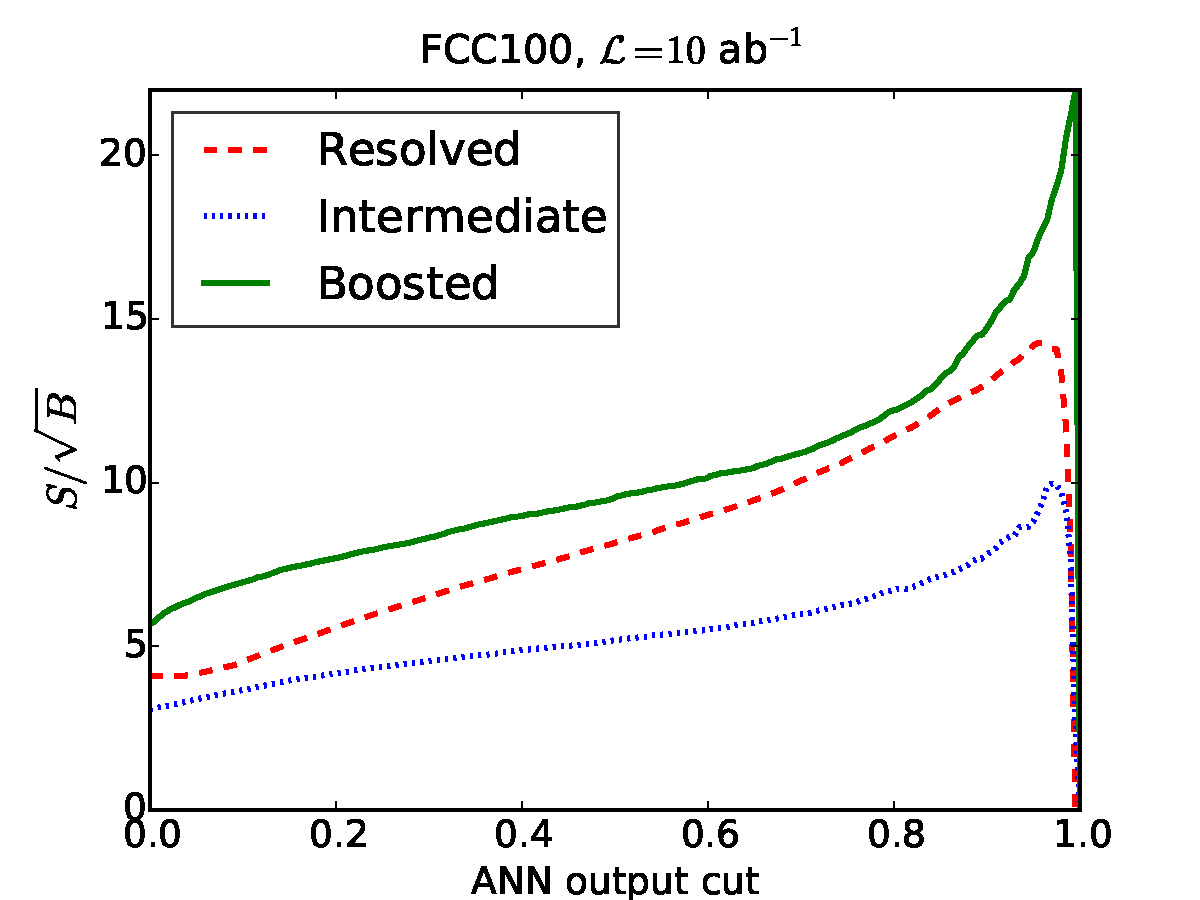
\includegraphics[width=0.48\textwidth]{plots/ssb_FCC100_4b.pdf}
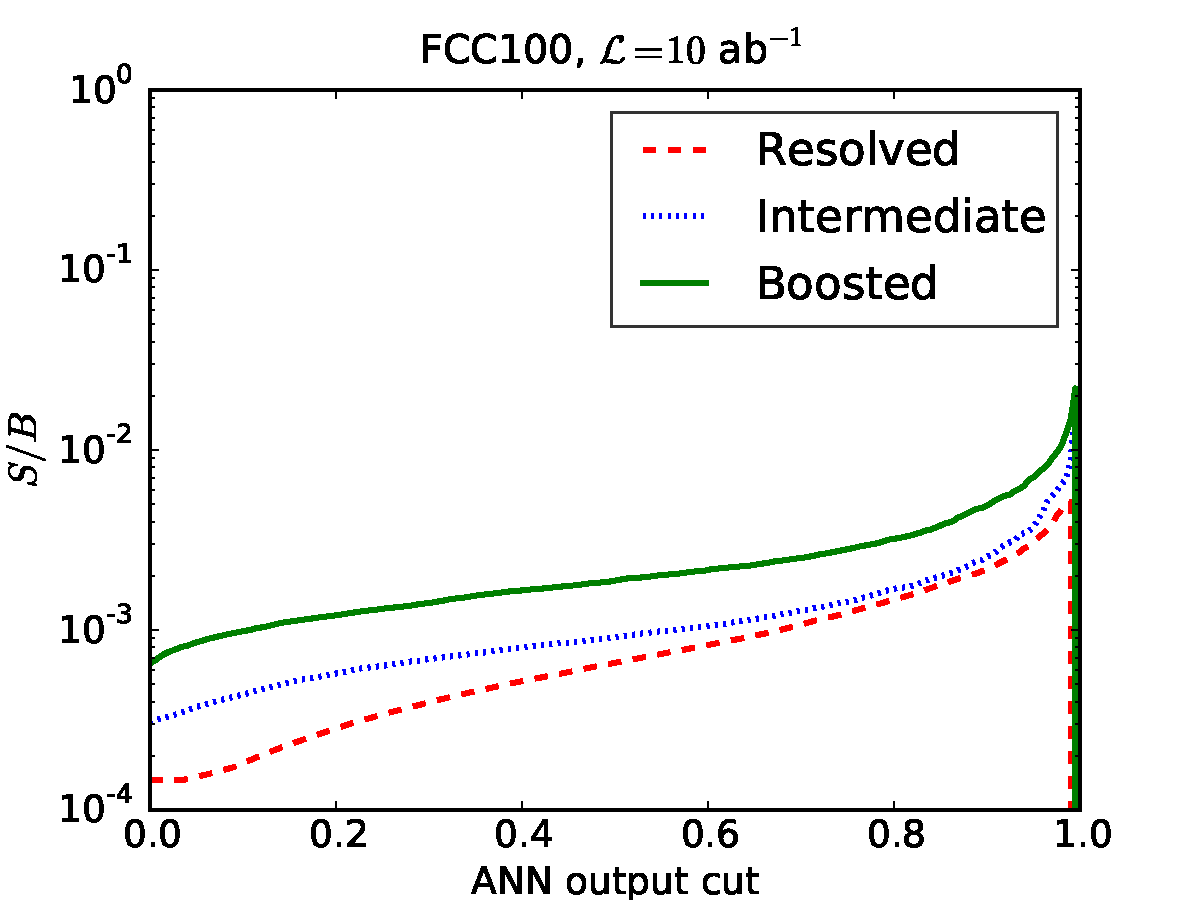
\includegraphics[width=0.48\textwidth]{plots/sb_FCC100_4b.pdf}
\caption{\small
  The values of the signal significance, $S/\sqrt{B}$, and of the
  signal over background ratio, $S/B$, for the boosted, intermediate
  and resolved categories as a function of the cut
  $y_{\rm cut}$ in the ANN output.
  %
  Only the $4b$ QCD background is considered here.
  %
  The $y_{\rm cut}=0$
  results are those at the end of the cut-based
  analysis. 
}
\label{fig:sb_mva}
\end{center}
\end{figure}
%%%%%%%%%%%%%%%%%%%%%%%

The results for the signal significance $S/\sqrt{B}$ and
the signal over background ratio
$S/B$ at a 100 TeV collider as a function of the ANN output cut $y_{\rm cut}$
for the three categories are shown in 
Fig.~\ref{fig:sb_mva}.
%
We have assumed a total integrated luminosity of $\mathcal{L}=10$ ab$^{-1}$, and only the
irreducible QCD $4b$ background is included.
%
The values 
for $y_{\rm cut}=0$ correspond to those at
the end of the loose cut-based analysis.
%
We observe how in the three
 categories there is a marked  improvement both in signal
 significance and in the signal over
 background ratio as compared to the pre-MVA results.
 %
 In Table~\ref{table:cutflowMVA} we collect
 the post-MVA results for the optimal value of the
    ANN discriminant $y_{\rm cut}$ in the three categories, compared with the
    corresponding
    pre-MVA results ($y_{\rm cut}=0$).
    %
    We also quote the number of signal and
    background events expected for an integrated
    luminosity of $\mathcal{L}=10$ ab$^{-1}$.



%%%%%%%%%%%%%%%%%%%%%%%%%%%%%%%%%%%%%%%%%%%%%%%%%%%%%%%%%%%%%%%%%%%%%%%%%%%%
\begin{table}[t]
  \centering
  \begin{tabular}{|c|l|c|c|c|c|}
    \hline
    \multicolumn{6}{|c|}{FCC100, $\mathcal{L}=10$ ab$^{-1}$} \\
    \hline
    \hline
    Category  &   &  $N_{\rm ev}$ signal &  $N_{\rm ev}$ back  &  $S/\sqrt{B}$ & $S/B$ \\ 
    \hline
    \hline
    \multirow{2}{*}{Boosted} &  $y_{\rm cut}=0$  &       $5\cdot 10^4$    &   $8\cdot 10^7$        &  6        &    $6\cdot 10^{-4}$         \\
    &  $y_{\rm cut}=0.99$ &   $2\cdot 10^4$    &  $1\cdot 10^6$         &      22    &    0.02     \\
    \hline
    \hline
    \multirow{2}{*}{Intermediate} &  $y_{\rm cut}=0$  &   $3\cdot 10^4$     & $1\cdot 10^8$  & 3   &  $3\cdot 10^{-4}$ \\
       &  $y_{\rm cut}=0.98$ &         $2\cdot 10^4$       &  $2\cdot 10^6$   &  10   & 0.007         \\
    \hline
    \hline
      \multirow{2}{*}{Resolved} &  $y_{\rm cut}=0$  &  $1\cdot 10^5$      & $8\cdot 10^8$  &   4  & $1.0\cdot 10^{-4}$  \\
    &  $y_{\rm cut}=0.95 $ &    $6\cdot 10^4$    &   $2\cdot 10^7$        &    15      &    0.004     \\
    \hline
      \end{tabular}
  \caption{\small Post-MVA results, for the optimal value of the
    ANN discriminant $y_{\rm cut}$ in the three categories, compared with the
    corresponding
    pre-MVA results ($y_{\rm cut}=0$).
    %
    We quote the number of signal and
    background events expected for $\mathcal{L}=10$ ab$^{-1}$,
    the signal significance $S/\sqrt{B}$ and
    the signal over background ratio $S/B$.
    %
    Only the QCD $4b$ background is considered here.
    %
    \label{table:cutflowMVA}
  }
\end{table}
%%%%%%%%%%%%%%%%%%%%%%%%%%%%%%%%%%%%%%%%%%%%%%%%%%%%%%%%%%%%%%%%%%%%%%%%%%%%


From Fig.~\ref{fig:sb_mva} and Table~\ref{table:cutflowMVA} we observe that the statistical
significance of the three categories is very large, with a post-MVA value of
$S/\sqrt{B}\simeq 20$ in the boosted
category.
%
However, we also find that as compared to 14 TeV, the QCD multijet background increases
more rapidly than the signal, and thus $S/B$ is actually smaller than at 14 TeV~\cite{Behr:2015oqq}.
%
Achieving  percent values in $S/B$ requires a very hard cuts on the value of the ANN output.
%
We observe that at 100 TeV the boosted category is the most promising one: not only
it benefits from the highest signal significances, it also exhibits
the best signal over background ratio.
%
Let us recall that at 14 TeV instead~\cite{Behr:2015oqq}  the higher significance was obtained with the resolved category.
%
Unfortunately, as we discuss below, the boosted category is the less sensitive to the Higgs self-coupling,
and thus a measurement of the trilinear will depend to good extent on the resolved category.
%
Therefore, at a 100 TeV collider, even more that at 14 TeV, the feasibility of the measurement
of $\sigma(hh\to b\bar{b}b\bar{b})$ depends strongly on how small the systematic
uncertainties can be, in particular for the background determination.

\paragraph{Extracting the Higgs self-coupling.}
%
The extraction of the trilinear coupling $\lambda$ from the
  corresponding cross-section is complicated by the
  destructive interference
  between diagrams that depend on $\lambda$ and those that do not.
  %
 Here we provide a first estimate of the accuracy
  in Higgs self-coupling extraction from the $b\bar{b}b\bar{b}$ final state
  that can be achieved at a 100 TeV hadron collider.
  %
  A robust estimate  would require
  a careful study of the impact of
  experimental systematic uncertainties, which is beyond the scope of this contribution.
  %
  Therefore, we will use a number of simplifying assumptions, in particular
  a very simple estimate of the total systematic uncertainty in the cross-section
  measurement, which is the limiting factor in the extraction of $\lambda$.

  The sensitivity in the Higgs self-coupling is defined by the $\chi^2$ estimator
  \be
  \label{eq:chi2profile}
  \chi^2(\lambda) \equiv \frac{\lc \sigma(hh,\lambda) - \sigma(hh,\lambda_{\rm SM})
    \rc^2}{\lp \delta_{\rm stat}\sigma\rp^2+\lp \delta_{\rm sys}\sigma\rp^2 } \, ,
  \ee
  where $\lambda$ is the Higgs
  self-coupling, $\lambda_{\rm SM}$ is the SM value, $\sigma(hh,\lambda)$ is the
  post-MVA signal cross-section for a given value of $\lambda$, and $\delta_{\rm stat}\sigma$ and
  $\delta_{\rm sys}\sigma$ are respectively the statistical and systematic uncertainties in the cross-section
  measurement.
  %
  Signal samples for a range of $\lambda$ values have been  processed
  by the same analysis chain, including the MVA (which is not
  retrained), than the SM samples.
  %
  The 68\% CL range for the extraction of $\lambda$ can then be found using
  the usual parameter-fitting criterion by determining the values $\pm \delta\lambda$
  for which the cross-section satisfies
  \be
  \label{eq:condition}
\chi^2(\lambda_{\rm SM}~^{+\delta\lambda}_{-\delta\lambda})=\chi^2(\lambda_{\rm SM})+1 \, .
\ee
%
The final result for the accuracy in the trilinear extraction can be obtained by combining
in quadrature the separate results
from the three exclusive categories.

In Fig.~\ref{fig:chi2} we show the $\sigma(hh\to b\bar{b}b\bar{b})$ cross-section at
  various steps of the cut-flow, including after $b$-tagging
  (before MVA) and after the MVA, in the resolved (left plot)
  and boosted (right plot) categories,  as a function of the Higgs self-coupling
  $\lambda/\lambda_{\rm SM}$ in units of the SM coupling.
  %
  See~\cite{Behr:2015oqq} for the definition of the different steps
  in the analysis chain.
  %
  We find that, despite that fact that the MVA is only trained on the SM sample, the signal
  selection efficiency of the MVA is relatively flat when $\lambda$ is varied, reflecting the fact
  that the signal kinematics do not change dramatically.
  %
  We also see that the resolved category (low and medium Higgs $p_T$) is more sensitive to variations of $\lambda$ than
  the boosted one (large Higgs $p_T$), as indicated by the shallower minimum of the latter after the MVA.
  %
  This reflects the well-known fact that the triangle diagram (which depends on the Higgs self-coupling) is
  dominant near the threshold region.
 

%%%%%%%%%%%%%%%%%%%%%%%%
\begin{figure}[t]
\begin{center}
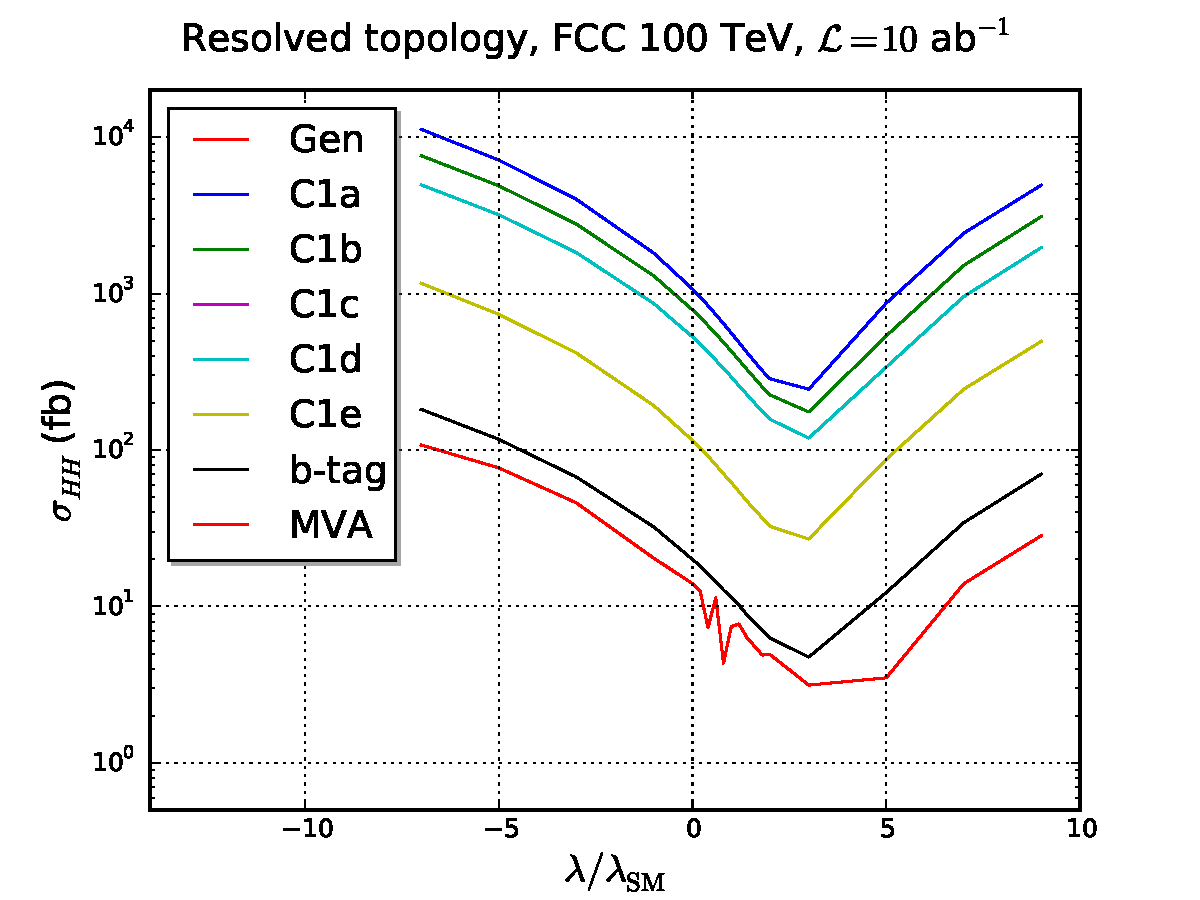
\includegraphics[width=0.48\textwidth]{plots/res_xSec_100TeV.pdf}
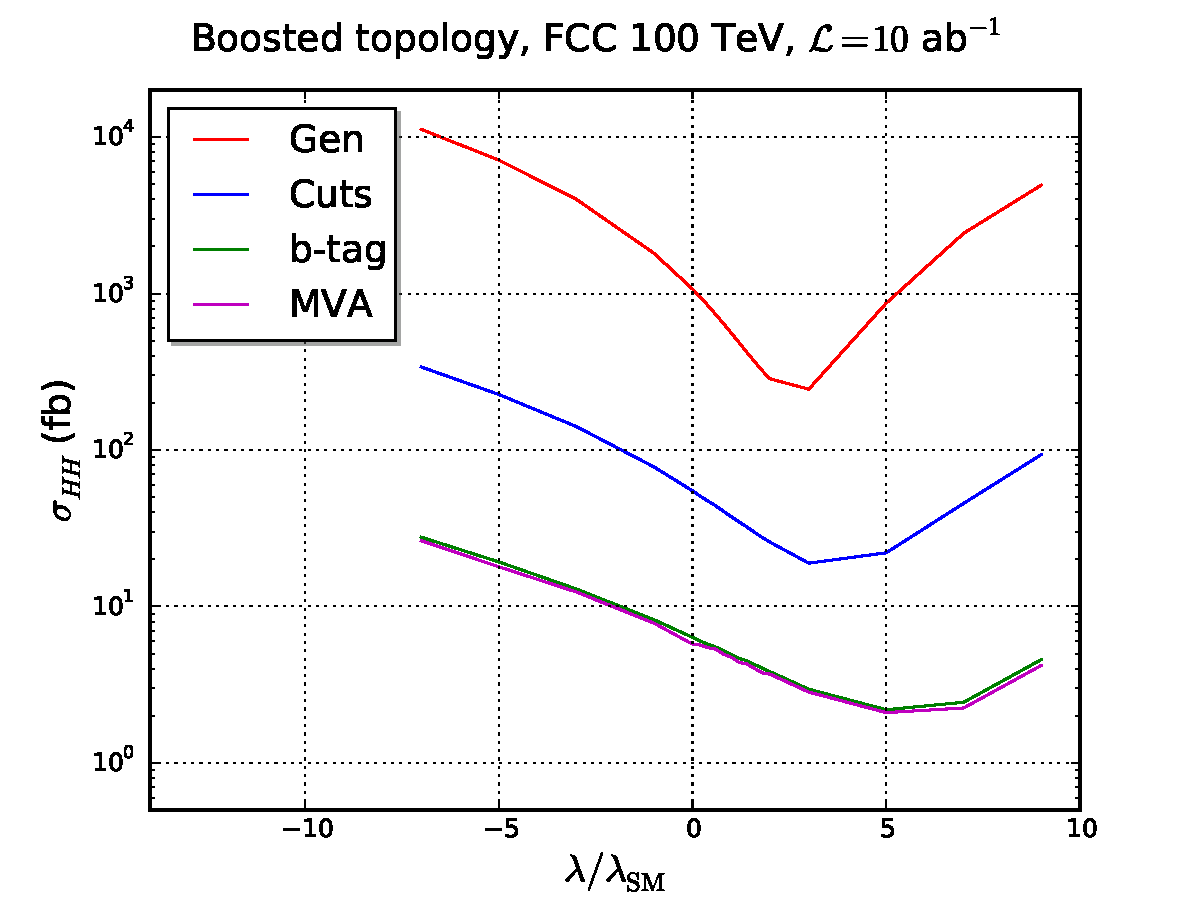
\includegraphics[width=0.48\textwidth]{plots/bst_xSec_100TeV.pdf}
\caption{\small
  The $\sigma(hh\to b\bar{b}b\bar{b})$ cross-section at
  various steps of the cut-flow, including after $b$-tagging
  (before MVA) and after the MVA, in the resolved (left plot)
  and boosted (right plot) categories, as  as a function of the Higgs self-coupling
  $\lambda/\lambda_{\rm SM}$ in units of the SM coupling.
}
\label{fig:chi2}
\end{center}
\end{figure}
%%%%%%%%%%%%%%%%%%%%%%%

 %
  Imposing the condition Eq.~(\ref{eq:condition}) we can derive the 68\% confidence level intervals
  on the Higgs self-coupling $\lambda_{\rm min}/\lambda_{\rm SM}$ (in units of the SM value) in the boosted, resolved and intermediate categories, for  different assumptions on the total systematic error in the measured
  cross-section.
  %
  The ranges that are found are reported in Table~\ref{tab:chi2}.
  %
  As expected, the results depend very strongly on the assumption for the systematic uncertainty
  on the measured cross-section.
  %
  In the optimistic scenario of a measurement with $\delta_{\rm sys}\sigma=25\%$,
  the best performance comes from the resolved category, where at the 68\% CL the trilinear
  can be determined to lie in the interval $\lambda/\lambda_{SM}\in \lc 0.9, 1.5\rc$.
  %
  Looser constrains are derived from the intermediate and specially from the boosted category.
  %
  On the other hand, for $\delta_{\rm sys}\sigma=100\%$, the constraints in all three categories
  become very loose, specially for $\lambda/\lambda_{\rm SM}\ge 1$, due to the negative interference effects.

  %%%%%%%%%%%%%%%%%%%%%%%%%%%%%%%%%%%%%%%%%
\begin{table}[h]
  \centering
  \begin{tabular}{|c|c|c|}
    \hline
  $\lc \lambda_{\rm min}/\lambda_{\rm SM},\lambda_{\rm max}/\lambda_{\rm SM} \rc$  &  $\delta_{\rm sys}\sigma=25\%$ & $\delta_{\rm sys}\sigma=100\%$ \\
    \hline
    \hline
Boosted   & $\lc -0.1, 2.2\rc$  & $\lc -1.5, > 9\rc$  \\
\hline
Intermediate   & $\lc 0.7, 1.6\rc$  &  $\lc -0.4, > 9\rc$  \\
\hline
Resolved   & $\lc 0.9, 1.5\rc$  &  $\lc -0.1, 7\rc$  \\
\hline
  \end{tabular}
  \caption{\small \label{tab:chi2} The 68\% confidence level intervals
    on the Higgs self-coupling $\lambda_{\rm min}/\lambda_{\rm SM}$ (in units of the SM value)
    obtained from the condition
    Eq.~(\ref{eq:condition}) in the boosted, resolved and intermediate categories.
    %
    We consider two different assumptions on the total systematic error in the measured
    cross-section,  $\delta_{\rm sys}=25\%$ and $\delta_{\rm sys}=100\%$.
  }
\end{table}
%%%%%%%%%%%%%%%%%%%%%%%%%%%%%%%%%%%%%%%%%%%%%%%%%%%%%%%%
  
\paragraph{Summary.} In this contribution we have performed a first exploration of the accuracy that can be expected
for the extraction of the Higgs self-coupling at a 100 TeV hadron collider using the $b\bar{b}b\bar{b}$ final state.
%
We find that while the statistical significance of the measurement of the $\sigma(hh\to b\bar{b}b\bar{b})$ cross-section
is very large, the $S/B$ ratio is quite low (and in particular worse than at 14 TeV),
specially in the resolved category, the one with the highest sensitivity
to the self-coupling.
%
This is a consequence of the fact that from 14 TeV to 100 TeV the QCD multijet background increases more rapidly than
the di-Higgs signal.
%
Our estimate of the expected precision on the Higgs trilinear depends strongly on the assumptions
about the experimental systematics.
%
For a measurement with a 25\% systematic uncertainty, the self-coupling can be determined
with accuracy $^{+50\%}_{-10\%}$ at the 68\% CL using the resolved category, but these constraints become substantially
looser if the systematic uncertainties are increased.

%%%%%%%%%%%%%%%%%%

\bibliography{HH4b}



\end{document}
